\documentclass[a4paper]{report}

\usepackage{masterThesisEn}
\usepackage{graphicx}
\usepackage{xspace}
\usepackage{multirow}
\usepackage{url}
% [required] Title:\maintatile{title}
\maintitle{A study on time series topic popularity extraction methods with topic modeling
}

% [required] Published date:\publish{year}{month}
\publish{2020}{July}

% [required] Student ID:\student{ID number}{Name}
\student{201826098}{Khan Muhammad Haseeb UR Rehman}

% [required] Abstract:\abst{abstract}
\abst{
Topic modeling is extensively used for the natural language processing (NLP) problems of summarizing, organizing, and understanding large document datasets. Latent Dirichlet Allocation (LDA) is widely used for the collection of topics, whereas Dynamic Topic Model (DTM) is famous for the time-series topic analysis. However, by estimating the number of occurrences of topics in each time slice, we can obtain time-series topic popularity using standard LDA. Therefore, if this can be extracted with LDA, then why do we need DTM which has a very high computation cost? The purpose of this research is to determine, either time-series topic information can be extracted from LDA or we need DTM. Topic drifting and popularity are two fundamental aspects of time-series topic analysis. We conducted experiments with multiple datasets to check the reliability of the information extracted from both models. We used Jensen-Shannon (JS) similarity-based analysis to check for information overlap, also overall and time-series correlation analysis as an inverse approach to extract DTM information from LDA topics. Lastly, we constructed time-series topic popularity graphs for both models from the document-topic distributions and compared the results. Our results show that there is notable DTM topic drifting information in some cases and sometimes no or vague topic drifting. Topic drifting embedded in DTM topics makes this model less favorable for topic popularity analysis. On the other hand, LDA topics with no time transition information provided concrete results of topic popularity. Thus, our results favor the usage of LDA.
}

% [required] Academic advisors:\advisors{Principal}{Secondary}
\advisors{Atsuyuki Morishima}{Kei Wakabayashi}


% output
\begin{document}

\makecover

\addtolength{\textheight}{-5mm}
\setlength{\footskip}{15mm}	% set footer
% List of contents/figures

\justifying

%\addtolength{\topmargin}{-20mm}

\fontsize{11pt}{15pt}\selectfont

\pagenumbering{roman} % I, II, III, IV 
\tableofcontents
\listoffigures

% contents
\parindent=2em	% set indent
\pagebreak\setcounter{page}{1}
\pagenumbering{arabic} % 1,2,3
\pagestyle{plain}

% chapter:\chapter{}
% section:\section{}
% subsection:\subsection{}

\chapter{Introduction}
Latent Dirichlet Allocation (LDA) \cite{blei2003latent} and Dynamic Topic Model(DTM) \cite{blei2006dynamic} are widely used topic models that revolutionized the solving of unsupervised topic modeling-based NLP problems.
Situations that need the assistance of topic models often involve time-series document collections, including Twitter posts, news articles, and academic paper archives, because a continuous accumulation of documents typically yields a massive amount of text data.
By focusing on the nature of time-series, many useful applications can be developed, such as bursty topic detection \cite{koike2013time}, trend analysis \cite{kawamae2011trend,zhang2015market,khan2019events}, topic evolution analysis \cite{blei2006dynamic,kalyanam2015context,xie2016topicsketch,amoualian2016streaming,acharya2018dmdtm}, and topic transition pattern mining \cite{kim2015toptrak}, etc.

To capture the time-series features of topics, DTM and its related-models \cite{amoualian2016streaming,acharya2018dmdtm} assume dynamic drift of distributions.
Although the DTM-based models appropriately find topics over time, they require expensive computational cost, which can be a critical drawback in some applications.
On the other hand, there is a large body of work developing efficient inference algorithms for LDA because of its simpler architecture compared to DTM.
While both models learn and work differently and even give different results, some practitioners and researchers employ LDA instead to analyze the time-series nature to take advantage of its efficiency, and these attempts seem to be successful according to the literature \cite{khan2019events}.

The question that arises in this background is; if time series topics information can be extracted by using LDA, which is faster than DTM, then why do we need to use DTM?
To answer the above-mentioned question this research is conducted with a problem statement that "\emph{Can time-series topic information of DTM be extracted from LDA?}"
To the best of our knowledge, there have been no studies that extensively compared the information extracted using LDA with that of DTM.

In this paper, we examine the differences between LDA topics and DTM topics by using multiple datasets and model configurations.
For this, we must compare two sets of topics from both models. Topic drifting and topic popularity are fundamental time-series information that can be extracted from DTM. Topic drifting is the topic transition over time and popularity is the measure of topic proportion at each time slice. The challenging part in topic transition analysis is that, DTM topic set has a sequential structure whereas LDA topic set has no type of sequential information. To map the unstructured topic set with DTM topics, we used a probability distribution similarity method.

Based on this matching, we analyzed both topic sets and in this process, we encountered with fragmentation issue, which we will describe later (\textbf{Figure \ref{fig:fragmentation}}).
DTM provides the time evaluation of topics, which means one single DTM topic can shift to a new subject if compared with the initial time's topic subject, where as an LDA topic's theme remains the same because LDA has no time aspect. This shifting in DTM topics is called fragmentation. In this experiment, we found that some DTM topics contain the information of two or more LDA topics; in other words, they have two or more fragmented topics.

To extract topic drifting from LDA topics, we compared both models, trying different approaches including correlation analysis and time-series topic correlation. For topic popularity, we built time-series population graphs for the topics of both models. Because both models have different types of information, there are pros and cons for each model. LDA extracts the focus on the collection of topics, whereas DTM can find connections between different themes and how subjects interchange within the same domain or topic.

Even though DTM has the edge of finding topic transitions over time for time-series data, in most cases, constructing only population graphs for LDA topics is enough for time-series analysis (e.g., events insights extraction from social media documents \cite{khan2019events}).
Some specific problems in which topic transition extraction is mandatory requires DTM despite its high computation cost (e.g., determining the focuses and trends of protected technological innovations across the entire disease landscape \cite{huang2019technological}).

\chapter{Related Work}
Koike et al. \cite{koike2013time} proposed a method that draws a time-series graph to find the bursty topic detection in Twitter data individually, as well as with correlated news, by using DTM \cite{blei2006dynamic}. They applied DTM to extract 50 topics from a subset of news articles and Twitter about \textit{The London Olympics}. Khan et al. \cite{khan2019events} performed a similar type of experiment using LDA. In their experiment, LDA was trained on 1000 topics on hashtag-pooled documents of English tweets. The dataset used in that research was Tweets2011 %\footnote{\url{https://trec.nist.gov/data/tweets/}}. 
They then created an inference dataset from the same dataset using day-hashtag tweet pooling. In the end, they created time-series graphs of topics that showed the topic popularity, topic burstiness, and interval of bursty topics. They explained the purpose of using LDA as follows: \emph{"Even though DTM allows the distribution of topics and words to be changed over time, DTM has a drawback in the computational cost, which particularly prevents to increase the number of topics K to hundreds or thousands. In Twitter, it's believed that there are many diverse topics including almost anything the people talk in their life. Consequently, the limitation of the DTM is a critical issue for the extraction of topics from Twitter."} In general, Koike et al.'s research and Khan et al.'s research are the same but use different topic models. we want to know why.

To understand this research better, we started with the basics: algorithms of both topic models. The main generative process of LDA with parameters $\alpha$ and $\beta$ is explained below and the implicit assumption is that documents are drawn interchangeably from the same set of topics.
\begin{enumerate}

\item For each document:
\begin{enumerate}
\item  Draw $\theta \sim Dir(\alpha)$
    \item For each word:
\begin{enumerate}
\item Draw $ Z \sim Mult (\theta) $
\item Draw $ W_{d, n} \sim Mult(\beta_z)$
\end{enumerate}
\end{enumerate}
\end{enumerate}

The logistic normal with mean $ \alpha $ to express uncertainty over proportions is part of DTM rather than the topic proportions $\theta$ drawn from Dirichlet distribution. Thus, DTM's generative process for slice $t$ of the sequential corpus is:

\begin{enumerate}
\item Draw topics $ \beta_t | \beta_{t-1}  \sim N(\beta_{t-1}, \sigma^2I) $
\item Draw $ \alpha_t | \alpha_{t-1}  \sim N(\alpha_{t-1}, \delta^2I) $
\item For each document:
\begin{enumerate}
\item Draw $ \eta \sim N(\alpha_t, a^2I)$
\item For each word:
\begin{enumerate}
\item Draw $Z \sim Mult(\pi(\eta)) $
\item Draw $W_{t,d,n} \sim Mult(\pi(\beta_{t,z})) $
\end{enumerate}
\end{enumerate}
\end{enumerate}

$\pi$ is a mapping factor that maps the multinomial natural parameters to the mean parameters, $\pi(\beta_{k, t})_w = \frac{exp(\beta_{k,t,w})}{\sum_{w'} exp(\beta_k,t,w')}$. For a detailed explanation, please refer to the following papers: LDA \cite{blei2003latent} and DTM \cite{blei2006dynamic}. Of note, even from just looking at the algorithms, we can see that the computational cost of DTM is much higher than LDA; this is the basis for this research.

Usually, documents are messy and can provide poor results when topic models are applied, so applying linguistic preprocessing may be of some help \cite{han2012automatically}. Topic models are not very efficient for short text documents, so tweet pooling is used for making relatively big documents for Twitter dataset. Tweet pooling has been proposed, and later proved experimentally \cite{mehrotra2013improving}, as an intuitive solution \cite{hong2010empirical,zhao2011comparing} when models perform poorly with a tweets dataset because of small document size.

Hashtag pooling is making documents based on hashtags where all the tweets with one hashtag form a single document. Any tweet having more than one hashtag is added to the tweet pool of each of those hashtags.  A new, under-examined but useful type of hashtag pooling known as day-hashtag pooling also greatly effects and helps for Twitter dataset in inference part. Day-hashtag pooling to some extent is a combination of hashtag pooling and temporal pooling proposed by Mehrotra et al. \cite{mehrotra2013improving} and even though author showed the possibility of hashtag-time pooling scheme but it is almost ignored in past. All the tweets with one hashtag on a specific date are grouped together to make one document.

\chapter{LDA Topics Inference}
To compare with DTM topics, the LDA topic information is organized by time series. We trained the LDA with different datasets without any modification to the LDA machinery.
Formally, when we denote a set of documents that we would like to analyze by $X = \{\mathbf{x}_1, \dots, \mathbf{x}_D\}$, we simply use $X$ as a training dataset for ordinary LDA training.

However, for the inference part that estimates the number of documents for each topic, we take the time information into account.
Each document $\mathbf{x}_d$ is associated to a specific time slice, which we denote by $\tau(\mathbf{x}_d)$.
Let $X_t = \{ \mathbf{x} \in $X$ | \tau(\mathbf{x}) =  t \}$ be a set of documents in time slice $t$.
We estimate the $\theta_{dk}$ for each document and estimate the number of documents for each topic $N_k^t$ at each time slice $t$ by the following equation:
\begin{equation}
N_k^t = \sum_{d: \mathbf{x}_d \in X_t} {\theta}_{dk}
\end{equation}
Specifically for a tweets dataset, we use day-hashtag pooling to make the documents and train the model on this document dataset. Thus, $N_k^t$ for this dataset can be calculated using the following equation:
\begin{equation}
N_k^t = \sum_{d: \mathbf{x}_d \in X_t} \theta_{dk} \times T_d
\end{equation}
where $N_k^t$ in Equation 2 is the estimated number of tweets of topic \textit{k} at \textit{t}, $\theta_{dk}$ is the probability of topic \textit{k} occurring in document \textit{d}, and $T_d$ is the total number of tweets in document \textit{d}.

Probability distribution $\mathbf{\theta}$ is calculated using Dirichlet distribution by applying LDA to the input data.

Given words $ \mathbf{x} = w_1, \dots , w_M$ we estimate the distribution of $\theta$.
\begin{equation}
p(\theta|\mathbf{x}) = \sum_\mathbf{z} p(\theta|z)p(\mathbf{z}|\mathbf{x})
\end{equation}
where corresponding topics $\mathbf{z} = z_1, \dots, z_K$ and the summation are over all possible assignments of $\mathbf{z}$. Since summation is analytically intractable, we apply Monte Carlo approximation with only one sample. We obtain a sample $ \hat{z} $ from $ p(z|x) $ using (collapsed) Gibbs sampling with five iterations. This approximation reduces the equation into the posterior probability of $ \theta $ given $ \hat{z} $.
\begin{equation}
p(\theta|x) \approx p(\theta|\hat{z})
\end{equation}
The posterior is a Dirichlet distribution of which the expectation $\hat{\theta}$ is:
\begin{equation}
\hat{\theta_k} = \frac{n_k + \alpha_k}{N + \sum_{k'} \alpha_{k'}}
\end{equation}
where $ n_k = \sum_{i=1}^N \delta(\hat{z_i}, k) $, i.e., the number of topic k in $\hat{z}$.

The final step is to estimate the number of documents to make the time-series popularity graphs.

\chapter{Similarity Analysis of DTM and LDA Topics}
The topics we get from both DTM and LDA are in the form of distributions. Along with the top words we also get the probability of occurrence of each word. An example of word distribution of a topic is shown in \textbf{Table \ref{table:topicDistribution}}, where the first element of the tuple is a word and the second element is the probability of this word in the current topic. We extract the top 50 words for all topics so word distribution is $K \times 50$ in LDA and $K$ is the number of topics. The top words may change in a DTM topic over time, so overall word distribution of a DTM topic varies, but it is $K \times 50 $ for one time slice, the same as an LDA topic. To check the relation between a DTM topic and an LDA topic, we use a simple but widely accepted similarity measure, the Jensen-Shannon(JS) divergence \cite{lin1991divergence}. For an LDA topic $T_{L}$ and DTM topic at time slice $t$ $T_{D}^t$, it is defined as:
\begin{equation}
JSD(T_L || T_D^t) = \frac{1}{2} D(T_L || T_{M}) + \frac{1}{2} D(T_D^t || T_{M})
 \end{equation}
 where
 \begin{equation}
  T_M = \frac{1}{2}(T_L + T_D^t)
 \end{equation}
 $D(T_L || T_{D})$ is the Kullback-Leibler divergence and can be calculated by below mentioned equation:
 \begin{equation}
D_{KL}(T_L || T_{D})  =  \sum_{w \in W} P(w| z_L) \log(\frac{P(w| z_L)}{P(w| z_D)})
 \end{equation}

 Only the top 50 words are considered for this similarity measure and word distributions do not sum up to one, so we apply normalization on both the DTM and LDA topic-word distributions.

\begin{table}[h!]
\begin{tabular}{|p{1cm}|p{13cm}|}
\hline \textbf{DTM}  &
('space', 0.0904)	('dimensional', 0.0492)	('nearest', 0.0346)	('data', 0.0341)	('projection', 0.0256)	('local', 0.0226)	('vectors', 0.0211)	('mapping', 0.0209)	('neighbor', 0.0159)	('maps', 0.0144)	('tangent', 0.0138)	('neighborhood', 0.0131)	('dimensions', 0.0125)	('dimension', 0.0122)	('dimensionality', 0.0122)	('feature', 0.0122)	('neighbors', 0.0114)	('points', 0.0097)	('kernel', 0.0091)	('point', 0.0091)	('coordinates', 0.0091)	('transformation', 0.0083)	('quantization', 0.0076)	('euclidean', 0.0074)	('projections', 0.0064)	('locally', 0.0064)	('manifold', 0.0062)	('structure', 0.0062)	('distances', 0.0059)	('reduction', 0.005)	('onto', 0.0048)	('spaces', 0.0048)	('nonlinear', 0.0044)	('topology', 0.0042)	('topological', 0.004)	('subspace', 0.004)	('directions', 0.0039)	('invariant', 0.0037)	('product', 0.0037)	('knn', 0.0036)	('coordinate', 0.0035)	('closest', 0.0034)	('matrix', 0.0031)	('mapped', 0.003)	('principal', 0.003)	('two', 0.003)	('multidimensional', 0.0029)	('laplacian', 0.0027)	('rbf', 0.0025)	('rotation', 0.0024) \\ \hline

\textbf{LDA} &
('inference', 0.034)	('map', 0.025)	('belief', 0.018)	('propagation', 0.018)	('message', 0.014)	('approximate', 0.012)	('product', 0.011)	('exact', 0.011)	('energy', 0.011)	('constraints', 0.01)	('partition', 0.01)	('marginal', 0.01)	('graphical', 0.01)	('sum', 0.009)	('probabilistic', 0.009)	('program', 0.008)	('assignment', 0.008)	('messages', 0.008)	('passing', 0.008)	('marginals', 0.008)	('field', 0.007)	('factor', 0.007)	('evidence', 0.007)	('potentials', 0.007)	('markov', 0.006)	('domain', 0.006)	('pairwise', 0.006)	('free', 0.005)	('factors', 0.005)	('potential', 0.005)	('fields', 0.005)	('mrf', 0.005)	('crf', 0.005)	('loopy', 0.005)	('approximations', 0.004)	('discrete', 0.004)	('constraint', 0.004)	('intelligence', 0.004)	('tractable', 0.004)	('ground', 0.004)	('ising', 0.004)	('lifted', 0.004)	('formula', 0.003)	('artificial', 0.003)	('logic', 0.003)	('weight', 0.003)	('configuration', 0.003)	('complexity', 0.003)	('represent', 0.003)	('original', 0.003) \\ \hline

\end{tabular}
\caption{Topic-word distribution of sample DTM and LDA topics}
\label{table:topicDistribution}
\end{table}

This JS analysis tells us about the information overlap between DTM and LDA topics and is a good way to confirm weather the  topics are similar in both models or that the topic-word distributions are totally different. This analysis also illustrates fragmentation. For example, the JS similarity measures changes between two or more LDA topics and a DTM topic over time. An example is shown in \textbf{Figure \ref{fig:fragmentation}}, where we see that the sample DTM topic was "Tensor decomposition for signal processing" in the starting years, but from 2005 onward the topic's theme shifted rapidly towards "Tensor decomposition" and "Signal processing" was no longer very significant. Whereas "Tensor decomposition" and "Signal Processing" are two different topics found in LDA analysis. This phenomenon is called fragmentation.

\begin{figure*}[t]
\begin{center}
\tiny
\begin{tabular}{|p{1.8cm}|p{1.8cm}|p{1.8cm}|p{1.8cm}|p{1.8cm}|p{1.8cm}|p{1.8cm}|}
\hline \bf T=0, (year = 1987) & \bf T=5, (year = 1992) & \bf T=10, (year = 1997) & \bf T=15, (year = 2002) & \bf T=20, (year = 2007) & \bf T=25, ( year = 2012) & \bf T=30, (year = 2017) \\ \hline

'matrix', 'vectors', 'components', 'component', 'analysis', 'principal', 'signals', 'signal', 'matrices', 'spectral', 'column', 'eigenvalues', 'source', 'orthogonal', 'eigenvectors', 'eigenvalue', 'row', 'diagonal', 'sources', 'pca', 'independent', 'subspace', 'separation', 'spectrum', 'columns', 'inverse', 'singular', 'wavelet', 'product', 'decomposition', 'algorithm', 'rows', 'coefficients', 'eigenvector', 'reconstruction', 'vector', 'natural', 'variance', 'projection', 'linear', 'blind', 'transform', 'oja', 'bell', 'mixing', 'ica', 'fourier', 'elements', 'correlation', 'covariance'
&
'matrix', 'component', 'components', 'analysis', 'principal', 'vectors', 'signal', 'source', 'signals', 'matrices', 'pca', 'sources', 'spectral', 'independent', 'separation', 'eigenvalues', 'eigenvectors', 'orthogonal', 'eigenvalue', 'column', 'row', 'diagonal', 'wavelet', 'algorithm', 'decomposition', 'subspace', 'singular', 'spectrum', 'blind', 'reconstruction', 'natural', 'columns', 'ica', 'inverse', 'mixing', 'rows', 'variance', 'product', 'coefficients', 'oja', 'bell', 'eigenvector', 'linear', 'projection', 'vector', 'transform', 'basis', 'covariance', 'non', 'mixtures'
&
'matrix', 'component', 'components', 'analysis', 'independent', 'source', 'signal', 'sources', 'separation', 'principal', 'ica', 'signals', 'pca', 'blind', 'matrices', 'wavelet', 'vectors', 'algorithm', 'natural', 'mixing', 'decomposition', 'eigenvalues', 'spectral', 'diagonal', 'subspace', 'eigenvalue', 'orthogonal', 'row', 'column', 'basis', 'singular', 'spectrum', 'eigenvectors', 'reconstruction', 'columns', 'variance', 'mixtures', 'bell', 'sensor', 'projection', 'rows', 'linear', 'coefficients', 'product', 'inverse', 'covariance', 'transform', 'kurtosis', 'non', 'eigenvector'
&
'matrix', 'signal', 'source', 'components', 'analysis', 'component', 'sources', 'signals', 'ica', 'matrices', 'independent', 'pca', 'separation', 'principal', 'subspace', 'vectors', 'basis', 'columns', 'eigenvalues', 'decomposition', 'wavelet', 'algorithm', 'reconstruction', 'variance', 'blind', 'column', 'diagonal', 'row', 'eigenvalue', 'orthogonal', 'sensor', 'mixing', 'spectral', 'eigenvectors', 'projection', 'rows', 'natural', 'spectrum', 'singular', 'rank', 'trace', 'entries', 'factorization', 'mixtures', 'norm', 'sparse', 'data', 'svd', 'diag', 'fourier'
&
'matrix', 'matrices', 'pca', 'rank', 'analysis', 'signal', 'components', 'source', 'columns', 'component', 'sources', 'reconstruction', 'subspace', 'ica', 'vectors', 'column', 'principal', 'signals', 'norm', 'trace', 'basis', 'row', 'low', 'entries', 'sparse', 'diagonal', 'decomposition', 'rows', 'factorization', 'independent', 'algorithm', 'error', 'eigenvalues', 'singular', 'projection', 'data', 'orthogonal', 'svd', 'eigenvalue', 'variance', 'diag', 'separation', 'fourier', 'eigenvectors', 'spectral', 'symmetric', 'sensor', 'bases', 'recover', 'elements'
&
'matrix', 'rank', 'matrices', 'norm', 'low', 'pca', 'subspace', 'tensor', 'columns', 'entries', 'column', 'principal', 'singular', 'decomposition', 'completion', 'analysis', 'vectors', 'sparse', 'factorization', 'error', 'data', 'component', 'trace', 'algorithm', 'reconstruction', 'spectral', 'row', 'rows', 'svd', 'diagonal', 'dictionary', 'recovery', 'basis', 'components', 'orthogonal', 'latent', 'projection', 'recover', 'sampling', 'observed', 'signal', 'eigenvalues', 'diag', 'method', 'robust', 'subspaces', 'vec', 'dimension', 'nuclear', 'time'
&
'matrix', 'rank', 'matrices', 'tensor', 'low', 'spectral', 'norm', 'subspace', 'decomposition', 'entries', 'error', 'singular', 'sparse', 'completion', 'pca', 'svd', 'vectors', 'columns', 'time', 'column', 'recovery', 'data', 'algorithm', 'analysis', 'factorization', 'phase', 'row', 'method', 'sampling', 'rows', 'diagonal', 'eigenvalues', 'initialization', 'signal', 'dimension', 'orthogonal', 'tensors', 'component', 'dictionary', 'principal', 'alternating', 'product', 'noise', 'ieee', 'projection', 'eigenvalue', 'nuclear', 'dimensional', 'power', 'recover'
\\ \hline

\end{tabular}
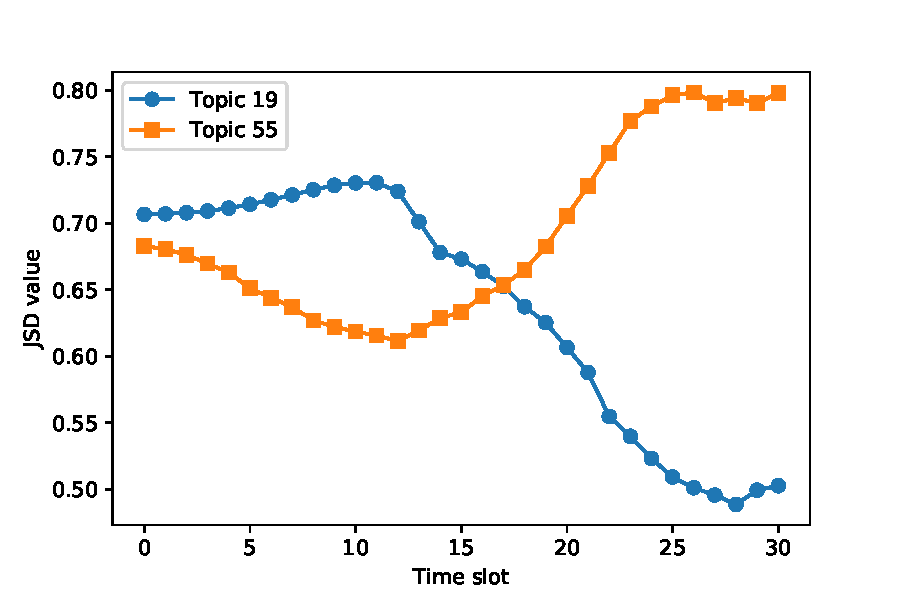
\includegraphics[scale=0.7]{JSgraph.pdf}
\tiny
\begin{tabular}{|p{7cm}|p{7cm}|}
\hline \bf LDA Topic 19 & \bf LDA Topic 55 \\ \hline

'rank', 'matrices', 'norm', 'tensor', 'entries', 'decomposition', 'columns', 'column', 'subspace', 'spectral', 'singular', 'completion', 'privacy', 'row', 'svd', 'trace', 'sparse', 'vectors', 'rows', 'private', 'product', 'diagonal', 'orthogonal', 'min', 'minimization', 'exact', 'factorization', 'differential', 'nuclear', 'symmetric', 'missing', 'entry', 'subspaces', 'recover', 'vec', 'tensors', 'arxiv', 'estimation', 'guarantees', 'noise', 'covariance', 'condition', 'power', 'projection', 'recovery', 'diag', 'norms', 'differentially', 'frobenius', 'k2f'
&
'noise', 'signal', 'components', 'component', 'filter', 'signals', 'source', 'filters', 'coefficients', 'mixture', 'noisy', 'sources', 'ica', 'separation', 'mixtures', 'filtering', 'variance', 'estimated', 'transform', 'blind', 'power', 'coding', 'wavelet', 'estimation', 'basis', 'snr', 'denoising', 'higher', 'invariant', 'gaussians', 'mixing', '1997', 'sensor', 'samples', 'unknown', 'orthogonal', 'fig', 'measurements', 'estimates', 'nonlinear', 'normalization', 'adaptive', 'overcomplete', 'equivalent', 'complex', 'correlated', 'elements', '2000', 'distributed', 'filtered'
\\ \hline

\end{tabular}
\caption{Models trained with the NeurIPS dataset with 60 topics for both DTM and LDA: Word distribution of DTM topic 0 at time slices T=0,5,10,15,20,25, and30 is shown in the first table. The last table shows the word distributions of LDA topics 19 and 55, respectively, and both curves in the graph are the JS similarity measure of DTM topic 0 with LDA topics 19 and 55. This is a graphical representation of two fragmented LDA topics related to one single DTM topic.}
\label{fig:fragmentation}
\end{center}
\end{figure*}

To extract DTM topic information from LDA, we use the inverse approach, which is to try to extract relevant information from LDA and, if the extracted information matches DTM's topics, then we can say that this technique is a good way to extract DTM's topics using LDA. For this comparison, we used different approaches.

\begin{itemize}
\item Overall correlation of LDA topics
\item Time-series topic correlation
\end{itemize}

Fragmentation means a single DTM topic contains two or more partial LDA topics. LDA topics that are related to a single DTM topic are similar in some aspect, so calculating the correlation among fragmented LDA topics is a good starting point. The correlation coefficient calculates the strength of the relationship between the relative movements of two variables, and the variables in this case are LDA topics that are calculated from the topics distribution $\theta_{dk}$. As DTM is time-dependent, it is better to also check the correlation of LDA topics in a series by categorizing documents with respect to time and then aggregating the correlation coefficient of each time slice.

Lastly, the time-series topic popularity, which is the second important information offered by DTM, can be extracted from the LDA topics. After calculating document-topic distribution $\theta_{dk}$. the documents are categorized with the same time-series information as used in DTM. Then, we calculate the estimated number of documents for each topic in a time series manner and construct a graph that is comparable to the DTM topics popularity information.

\chapter{Experiment}
The experimental process started with collecting and preparing the datasets. Then appropriate configurations for DTM and LDA models were selected. After training both models with one dataset set at a time, we extracted topics-word distributions and word probability. These word probabilities were used for computing the JS divergence from which we made the JS similarity-based graphs. We computed the overall correlation and time-series correlation for one of the datasets in one of the configurations to try to extract the DTM time-series topic distributions from the LDA topics. We also plotted population graphs from this configuration's inference part to compare it with the DTM topics.

\section{Datasets}
Three different datasets were used in this experimental procedure.

\textbf{NeurIPS}: This dataset consists of research papers from the conference of neural information processing systems(NeurIPS formally known as NIPS) from 1987, when the conference first started, to 2017. There are 7242 documents in this dataset with three unrecognizable, so a total of 7239 research papers were part of the dataset used in training the DTM and LDA.  In the preprocessing, we removed stop words (e.g., the, a, an, in) using the \textit{nltk.corpus}\footnote{\url{http://www.nltk.org/api/nltk.corpus.html}} python package, special characters (e.g., \$, @, \%, \&), URLs, and words having only two characters because most two characters words do not have concrete meanings (e.g, up, vs, ha).

\textbf{Twitter}: The second dataset is the Tweets2011 dataset of more than three million English tweets sampled between January 23 to February 8, 2011. As the original dataset consists of all the publicly available tweets in that period which means that the tweets are in many languages, we used the Python library \textit{langdetect}\footnote{\url{https://pypi.org/project/langdetect/}} to extract the English tweets. Usually, a tweet is a messy piece of text, so some preprocessing is desirable as the first step in cleaning this data.
We therefore removed stop words, usernames, URLs, special characters, and two-letter words. The next step was day-hashtag pooling. We obtained 408,200 documents after this pooling, which became part of the training dataset of the DTM and LDA.

\textbf{News}: This dataset\footnote{\url{https://components.one/datasets/all-the-news-articles-dataset/}} consists of 204,135 news articles from 18 American publications and each row has columns "id", "title", "author", "date", "content", "year", "month", "publication", "category", "digital", "section", and "url". Each row represents one single news article. Some of the entries may have a NULL value for this article. There are 191,530 articles that have date information and also the distribution of articles over the years is sparse. We therefore selected articles from 2016 and 2017, totaling 95,997 and 75,034 respectively. Thus, a total of 171,031 news articles were divided into 24 time slices based on the month-year parameter for DTM training and the inference of LDA. The same preprocessing steps were applied to this dataset as mentioned above for the other datasets.

\section{Models Configuration}
\textbf{LDA} implementing the stochastic variational Bayesian method of \cite{mimno2012sparse} in Java with three different numbers of topics $K$, 1000 docs per batch (also known as mini-batch size), and 1000 iterations was trained with the above-mentioned datasets one at a time.

\textbf{DTM} was implemented using the gensim.model.wrappers with DTM implementation \footnote{\url{https://github.com/magsilva/dtm}} in C and C++. We trained the DTM on three different numbers of topic configurations with each dataset.

\textbf{Topics:} We selected three values (30, 60, and 90) for the hyperparameter "number of topics", denoted as $K$. We trained the DTM and LDA with one dataset at a time and with one of the $K$ values.

The experiment environment was Ubuntu 16.04 for the operating system, two Intel 80n E5-2630 (2.40 GHz) with eight cores for the central processing unit, and Python and Java for the LDA implementation and Python and C/C++ for the DTM implementation.


\chapter{Results}
This section is divided into multiple sub-sections; each part explains the different aspects of our research.

\section{Training Time Cost}
As mentioned earlier, the computational cost for DTM is higher than LDA;  however, to determine the difference in training time, we conducted a small sub-experiment in which we trained both the DTM and LDA models with different-size documents and hyperparameter value $K$, which is the number of topics. The dataset used for this experiment was the "Twitter" dataset. Preprocessing cleaning and hashtag pooling were applied before training.

\begin{figure}[h!]
\begin{center}
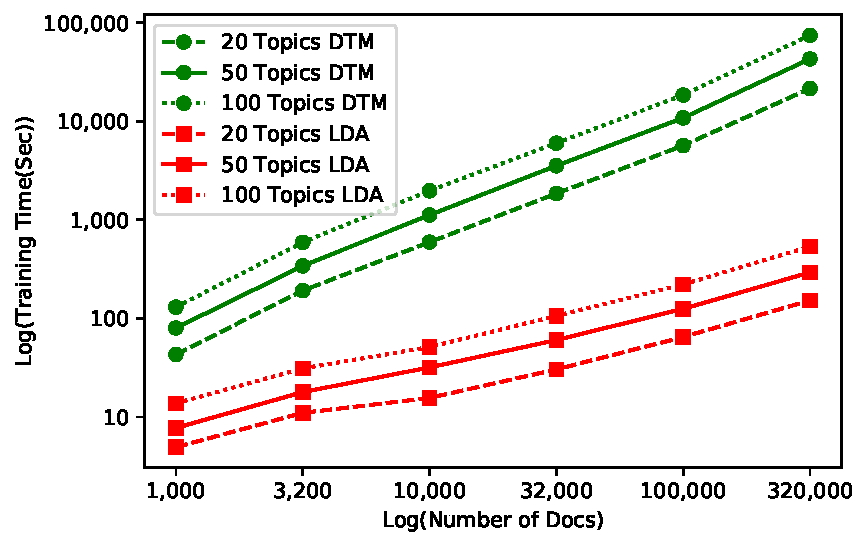
\includegraphics[scale=0.8]{costGraph.pdf}
\caption{This graph is in logarithmic scale to fit higher values into the figure. The x-labels are the number of documents on which the models were trained and y-axis is the time in seconds that each model took for training.}
\label{fig:trainingTime}
\end{center}
\end{figure}

\textbf{Figure \ref{fig:trainingTime}} shows that increasing the number of documents or the number of topics increase the training time. We see a roughly linear increase in time for both models. For small datasets, the training time of DTM was 10 times more than LDA and exceeds \textbf{"100 times"} for big datasets. Normally in NLP topic modeling problems, datasets are relatively bigger in size. We can therefore say that DTM will take around 100 times more time for training compared with LDA under the same conditions.

\section{Topic Drifting}
Topic drifting is fundamental information extracted from DTM. A single DTM topic consists of topics at each time slot. For clarity, let us call such a time-slice-topic the "focus" of the DTM topic. The focus of a DTM topic changes over time, as shown in the first part of \textbf{Figure \ref{fig:fragmentation}}, where the focus changed from "Signal Processing" to "Tensor Decomposition" by the end. This is called topic drifting or topic transition. We calculated the total unique vocabularies for each DTM topic. The minimum vocabulary size for any topic was 50. If any topic had $V_s$ close to this number, it means there were no new words in the different time slot topics. In short, the focus of this specific topic remained the same and there was no topic drifting.

\begin{table}[h!]
\begin{center}
\begin{tabular}{|c|c|c|c|c|}
\hline \textbf{Dataset} & \textbf{Topics} & $K(V_s > 70)$& $K(V_s > 90)$ & $K(V_s > 120)$ \\ \hline

\multirow{3}{*}{NeurIPS}  & 30 & 13 & 8 & 0 \\ & 60 & 58 & 56 & 11  \\ & 90 & 90 & 90 & 90  \\ \hline
\multirow{3}{*}{Twitter}  & 30 & 3 & 1 & 0 \\ & 60 & 3 & 0 & 0 \\ & 90 & 1 & 0 & 0 \\ \hline
\multirow{3}{*}{News}  & 30 & 29 & 20 & 5 \\ & 60 & 57 & 33 & 1 \\ & 90 & 83 & 37 & 2 \\ \hline

\end{tabular}
\caption{$V_s$ is the vocabulary size, which is the number of unique words that appeared in all time slot topic-word distributions of a single DTM topic. Minimum $V_s$ is 50.  $K(V_s > 70)$ means the number of DTM topics having a vocabulary size of more than 70. Similarly $K(V_s > 90)$ and $K(V_s > 120)$ mean the number of topics having a vocabulary size of more than 90 and 120, respectively. }
\label{table:topicDrifting}
\end{center}
\end{table}

In \textbf{Table \ref{table:topicDrifting}}, $K(V_s)$ values for the Twitter dataset are very low, which means there were not many new words in the DTM topics and the focus of the topics remained the same over all times. This implies that DTM topic drifting for the Twitter dataset is negligible. And $K(V_s)$ values for the DTM trained on NeurIPS and News dataset were relatively high, which implies that there were topic drifting phenomenons.

\section{JS Analysis}
To extract the information overlap of the DTM and LDA topics, we computed JS values using \textbf{Equation 6} for all the datasets in all topic configurations. The JS value is bounded by 0 and 1 for two distributions, where 0 means both distributions are identical and 1 means there is no similarity between both probability distributions. A threshold value of 0.7 was selected and any DTM topic distribution having a JS value lower than or equal to this threshold when measured with the LDA topic distributions was part of the related topic "RT", Fragmented topic "FT", and others. A summary of this analysis is set forth in \textbf{Table \ref{table:JStable}}.

\begin{table}[h!]
\begin{center}
\begin{tabular}{|c|c|c|c|c|c|c|}
\hline \textbf{Dataset} & \textbf{Topics} & \textbf{RT}& \textbf{FT} & \textbf{F 2} & \textbf{F 3} & \textbf{F 4 \& more} \\ \hline

\multirow{3}{*}{NeurIPS}  & 30 & 17 & 4 & 3 & 1 & 0 \\ & \textbf{60} & \textbf{42} & \textbf{16} & \textbf{11} & \textbf{5} & 0  \\ & 90 & 69 & 28 & 25 & 2 & 1 \\ \hline
\multirow{3}{*}{Twitter}  & 30 & 5 & 0 & 0 & 0 & 0 \\ & 60 & 11 & 1 & 1 & 0 & 0 \\ & 90 & 14 & 3 & 2 & 1 & 0 \\ \hline
\multirow{3}{*}{News}  & 30 & 8 & 1 & 1 & 0 & 0 \\ & 60 & 24 & 2 & 2 & 0 & 0 \\ & 90 & 42 & 4 & 4 & 0 & 0 \\ \hline

\end{tabular}
\caption{DTM and LDA trained on "Dataset with "Topics" configuration one at a time, "RT" is the total number of DTM topics having a relationship with the LDA topic/s. "FT", "F2", "F 3", and "F 4 \& more" are the number of DTM topics having a JS relationship with two or more LDA topics, only two LDA topics, only three LDA topics, and more than three LDA topics, respectively.}
\label{table:JStable}
\end{center}
\end{table}

\textbf{Table \ref{table:JStable}} shows that a negligible amount of "FT" fragmented topics was found for the datasets "News" and Twitter" because most news articles and tweets are instantaneous responses of some events, and these topics die within short period of time; in other words, we see other tweets and article about other events. Due to this focus shifting behavior of the documents, DTM cannot accurately locate topic transitions over time. That is why very few fragmented topics were found for these datasets. Related topics "RT" are comparatively higher for "News" as compared to "Twitter" dataset because the domain of tweets is huge; it could be anything ranging from personal (My pet is very cute) to political (US president announced a restriction on trade agreement with China), whereas the News articles domain is restricted compared with Twitter. We can therefore have many topics in the Twitter dataset and random initial conditions of both DTM and LDA. It is safe to say that both models could come up with different topics. As mentioned,  the News dataset domain is restricted so we see high topic overlapping values in this dataset's results.

The domain of the "NeurIPS" documents focused on a few subjects(machine learning, artificial intelligence, computational neuroscience, etc.), so related topics' "RT" values are very high compared with other dataset configurations. High fragmented topic "FT" values can be seen for the "NeurIPS" dataset in \textbf{Table \ref{table:JStable}} because research papers tend to follow previous researches or somehow align with previous research papers. That is why we can see a well-defined topic transitions in the DTM topics, as shown in \textbf{Fig \ref{fig:fragmentation}}.

In all the datasets, increasing the number of topics resulted in an increase in "RT" and "FT" values.

\begin{table}[h!]
\begin{center}
\begin{tabular}{|c|c|c|c|c|c|c|c|}
\hline \textbf{Dataset} & \textbf{DTM} & \textbf{LDA} & \textbf{RT}& \textbf{FT} & \textbf{F 2} & \textbf{F 3} & \textbf{F 4 \& more} \\ \hline

NeurIPS & 30 & 1000 & 25 & 20 & 3 & 7 & 10 \\ \hline

\end{tabular}
\caption{A special configuration with DTM topics and LDA topics was also examined to analyze the behavior of an LDA model trained with a high number of topics.}
\label{table:JS30DTM1000LDA}
\end{center}
\end{table}

If we increase the number of topics in LDA, we get more and more fragmented topics, which means that topics are further divided into smaller and more focused themes. DTM's computation cost restricts us from increasing the number of topics, so we cannot get the type of topics that we can get from LDA with a very high $K$ hyperparameter.

\section{Overall Correlation}
Due to fragmentation detection, being part of a single DTM topic, fragmented LDA topics should have some relationship with each other. For example, the documents that have a high probability of topic 0 shown in \textbf{Figure \ref{fig:fragmentation}} in the DTM analysis should have a high probability for topic 19 and 55 in the LDA analysis as compared to other topics. This phenomenon leads to the hypothesis that \textit{"fragmented topics have similar distributions"}. Therefore we find the overall correlation coefficient for all the fragmented topics extracted from the LDA model trained on the "NeurIPS" dataset with $K = 60$.
After training the model, topic distribution for each document was calculated using the method described in \textbf{Section 3}. This topic distribution gives us insights into the relevance of each topic with each topic. Document-topic probabilities of the fragmented topics were used as variables to calculated the overall correlation.

The analysis showed no significant results and most of the correlation values were around 0, which means there is no linear relationship between fragmented topics, with few exceptions ranging up till "0.44" indicating some relation but not significant enough to prove our hypothesis.

\section{Time Series Correlation}
We also checked the correlation in a time-series manner because fragmented topics have time-series effects. For example \textbf{Figure \ref{fig:fragmentation}} shows that the JS similarity for both topics was close until the 15th time slot and the DTM topic was biased towards topic 19 as compared to topic 55 around the end. It is also, therefore, worth checking the relationship of fragmented topics in a time-series manner to further explore our hypothesis.

We split the document-topic distribution according to the time slots, checked the correlation of the fragmented topics in each time slot, and then made a graph to view the correspondence of the time-series correlation graph with JS graphs. The resultant graphs showed no strong relationship between fragmented topics and we could not find evidence to prove our hypothesis \textit{fragmented topics have similar distributions}.

\section{Time Series Topic Popularity}
Topic popularity is the second fundamental information that can be extracted from a topic model and, especially in the case of DTM, time-series topic popularity is estimating the number of documents for each topic at each time slice. We can easily construct this information into a self-explanatory graphical representation of topic popularity. For this analysis, we selected the 60 topics of the "NeurIPS" configuration. Then $\gamma$ distributions for the documents were calculated which gives the probability of each topic for each document. Time-depended summation over the topics then gives us the estimated number of documents for each topic at each time slot. we can also extract this information from LDA with just a few extra steps. First, we trained the LDA with the same dataset and got topics with the same 60-topic configuration. Before getting the $\theta_{dk}$ distributions for the documents, we saved the date information with the documents so that when we got the $\theta_{dk}$ distributions, we knew the corresponding date of each document. With these distributions and dates, we applied time-dependent summation over the topics and got an estimated number of documents for each topic at each time slot. Afterward, we plotted this information into graphs. To reduce noise effects and to make the graphs smooth, we used the Savitzky-Golay digital filter.

\begin{figure}[h!]
\begin{center}
\begin{tabular}{cc}
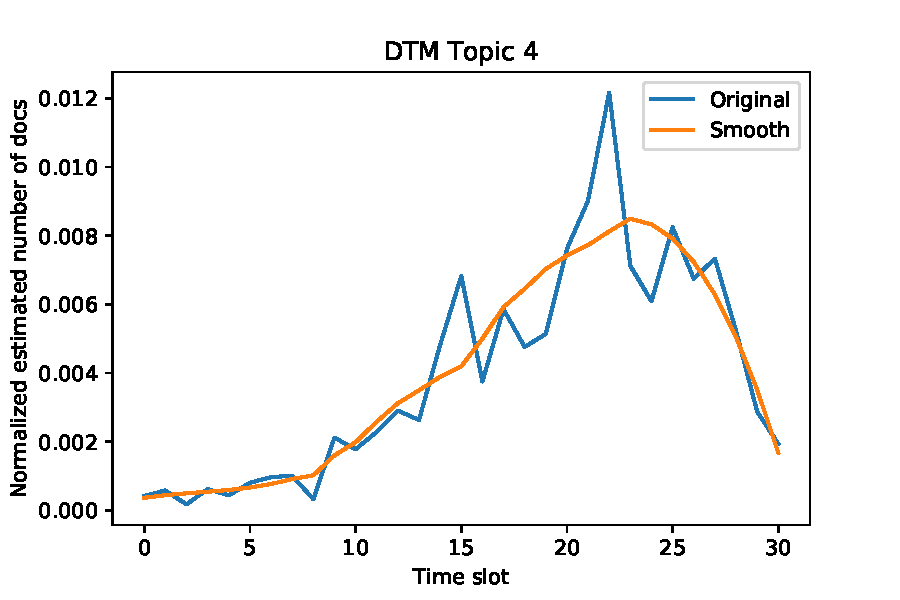
\includegraphics[scale=.5]{DTMpopulationTopic4.pdf} &
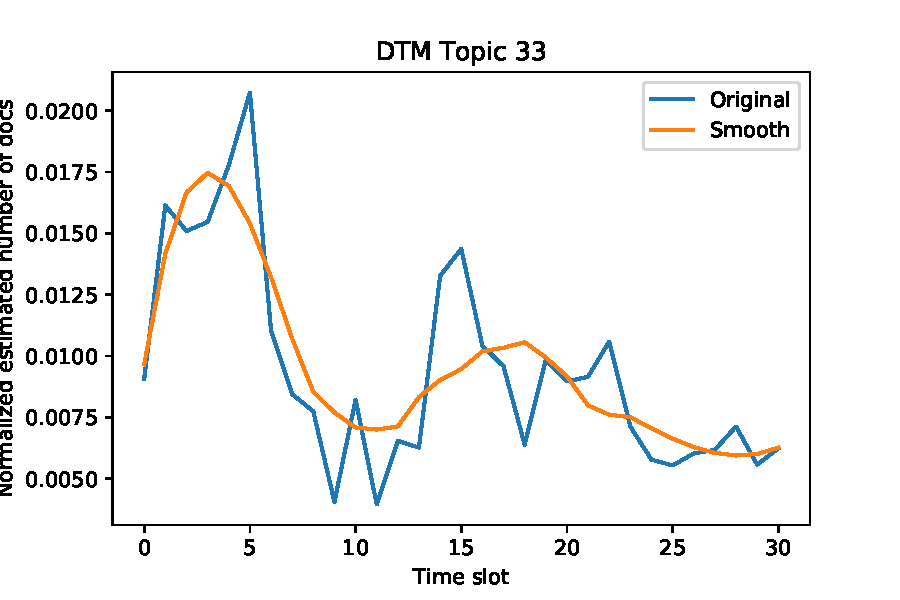
\includegraphics[scale=.5]{DTMpopulationTopic33.pdf} \\
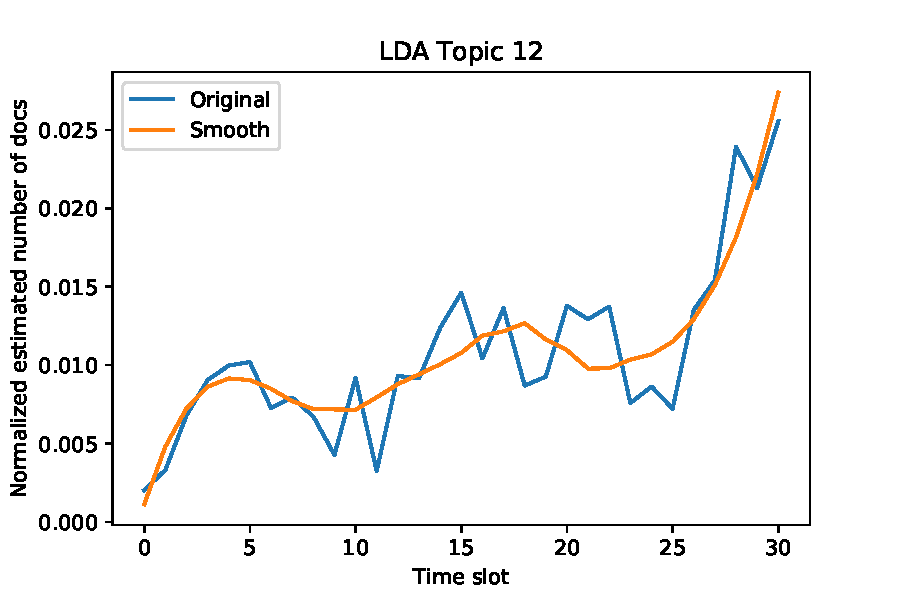
\includegraphics[scale=.5]{LDApopulationTopic12.pdf} &
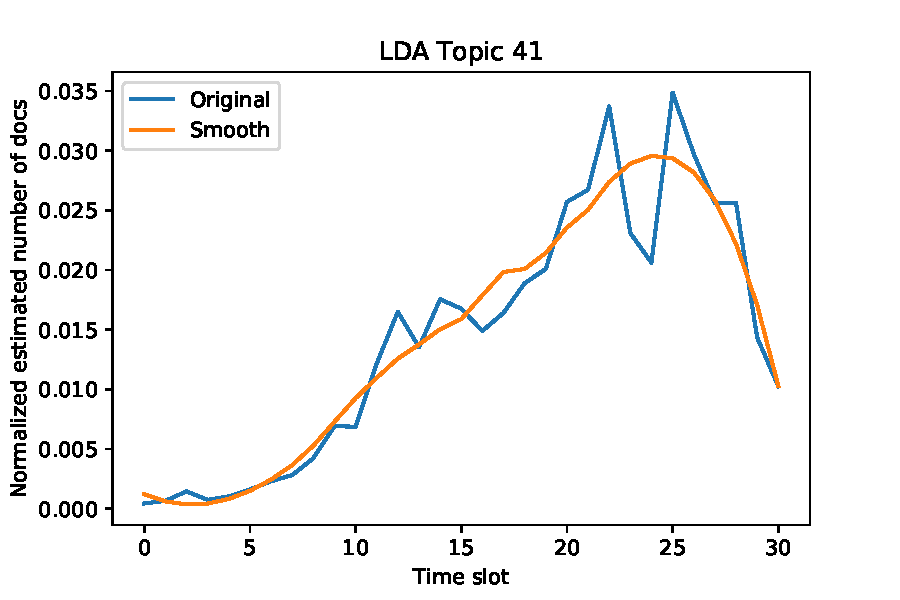
\includegraphics[scale=.5]{LDApopulationTopic41.pdf}
\end{tabular}
\caption{Number of documents for each time slot estimated from $\gamma$ and $\theta$ distributions of the documents for DTM and LDA respectively. Two topics from each model are shown here. The horizontal axis shows the time slot number and the vertical axis is the normalized estimated number of documents for these topics.}
\label{fig:populationGraphs}
\end{center}
\end{figure}


\textbf{Figure \ref{fig:populationGraphs}} shows the time-series topic popularity of both the DTM and LDA topics. The top two graphs in the figure are of DTM topics 4 and 33, respectively, and the bottom graphs show the time-series popularity of LDA topics 12 and 41. These graphs show that the time-series topic popularity can be extracted from DTM as well as LDA.


\chapter{Discussion}
 Topic drifting and time-series topic popularity are the main aspects of this research and we compared these aspects for DTM and LDA. In this section, we discuss a few important points of both concepts as they apply to DTM and LDA.

\textbf{Topic Drifting}: There is no topic drifting for DTM trained on the "Twitter" dataset({Table \ref{table:topicDrifting}}), so the only important information which can be extracted from such datasets is the time-series topic popularity which can be extracted using LDA, thus avoiding the high cost of using DTM as the topic model.  For the "NeurIPS" dataset, the topic drifting increased as we increased the number of topics for the DTM model. All 90 topics have  $V_s$ greater than 120 words for the NeuIPS data in the 90-topic configuration(Table \ref{table:topicDrifting}), which means there was high topic drifting and this high topic drifting information provides rich insights into topic transitions. Therefore, if we specifically want to examine topic drifting over time in such datasets, DTM is a promising model to use; however, we must keep in mind that if our goal is topic popularity, then LDA is a far better option. From the same table, we also see the drifting in the topics extracted from the "News" dataset, but the vocabulary size is comparatively low for the higher number of topics. This means that we have topics drifting with such datasets, but it may not be as effective as we want. More subjective analysis based on your problem can help determine if DTM is a good option or not. One interesting insight should be mentioned here; DTM tends to forcefully find the topic transitions in some cases. For example, in the 30-topic configuration for the News dataset, topic 29 started with words like \textit{(archive, team, collection, sign, projects, machine, contains, lost, providing, comment, websites, collections, wayback)}, but the word distribution at the end was \textit{(travel, airport, flight, air, trip, passengers, flights, travelers, plane, airlines, united, airline, passenger)}. Looking at these distributions, we can say that DTM failed to extract the correct topic drifting over time for topic 29.

\textbf{Topic Popularity} We have $\gamma$ and $\theta$ distributions for DTM and LDA, respectively. Once the model is trained, we can extract these distributions for any document and these distributions provide the topics proportion for each document. We can estimate the number of documents for each topic using the method described in Section 3 for the LDA model and, with this time-series document estimation, we can construct a time-series topic popularity graph. Similarly, we can construct this graph for DTM topics. Thus, this fundamental information can be extracted using both models. Notably, the topic popularity extracted from DTM is a little vague because DTM topics have topic transition information embedded within the topics. For example, topic 4 shown in Figure \ref{fig:populationGraphs} has word distribution \textit{(retrieval, content, query, queries, text, relevance, documents, semantic, words, document, lda, relevant, collection, word, latent, topics)} at T= 0, which is about "Information retrieval from documents" and the word distribution at T= 30 is \textit{(topic, topics, document, lda, word, documents, words, latent, dirichlet, text, models, allocation, model, corpus, gibbs, modeling, blei)}, which is about "Document analysis with LDA". Similarly, DTM topic 33 was about "Language structure rules" in initial time slots and the theme of the topic was changed to "Question-answer reasoning" around the end. Therefore, if we are looking for the popularity graph of a topic "Information Retrieval", then LDA topic 12 is a more accurate option. Similarly, LDA topic 41 is more accurate if we want to see the popularity graph of the topic "Variational topic model LDA" because there is no topic drifting in LDA. The word distribution for LDA topic 12 is \textit{(word, words, language, sequence, recurrent, text, lstm, rnn, semantic, context, attention, table, vectors, embedding, sequences)} and for LDA 41 is \textit{(latent, inference, topic, sampling, mixture, variational, posterior, gibbs, dirichlet, topics, lda, markov, document, likelihood, prior, distributions)}. Because of the topic transition information embedded with DTM topics, it is not the best option for time-series topic popularity information.


\chapter{Conclusion}
In this research,we executed a comprehensive study on the time-series analysis of the popular topic models DTM and LDA. Our research focused on the fundamental time-series information of topic drifting and topic popularity.To compare DTM and LDA, we tried to extract this information from the topic distributions of both models. Multiple datasets along with multiple topic configurations were used for this experiment. Our findings are:

\begin{enumerate}
\item DTM takes 100 times longer to train the model as compared than LDA for large datasets.

\item Topic drifting is a unique property of DTM that is difficult to extract from the LDA model, but some datasets like Twitter do not have topic transition information, so applying DTM to such datasets is a waste of resources.

\item Time-series topic popularity can be extracted from both models, but it is precise from LDA because DTM has topic transition embedded in the topics.
\end{enumerate}

 Fragmentation of topics was also detected in this process from the datasets focused on one domain, e.g., "NeurIPS", which is another interesting aspect of this research and could be studied in the future. To summarize, time-series topic popularity --common information needed as time series information-- should be extracted from LDA because it is faster and provides concrete information as compared to DTM. However, if topic drifting is required, then DTM is the only option, although it sometimes may give inaccurate information.

\chapter*{Acknowledgement}


% References
\newpage
\addcontentsline{toc}{chapter}{\numberline{}References}
\renewcommand{\bibname}{References}

%% for using bibtex
%\bibliographystyle{junsrt}
%\bibliography{hoge(.bib)}
\bibliographystyle{unsrt}
\bibliography{References}

\end{document}